\documentclass{standalone}
\usepackage{tikz}
\usepackage{pgfplots}
\pgfplotsset{compat=1.18}

\begin{document}
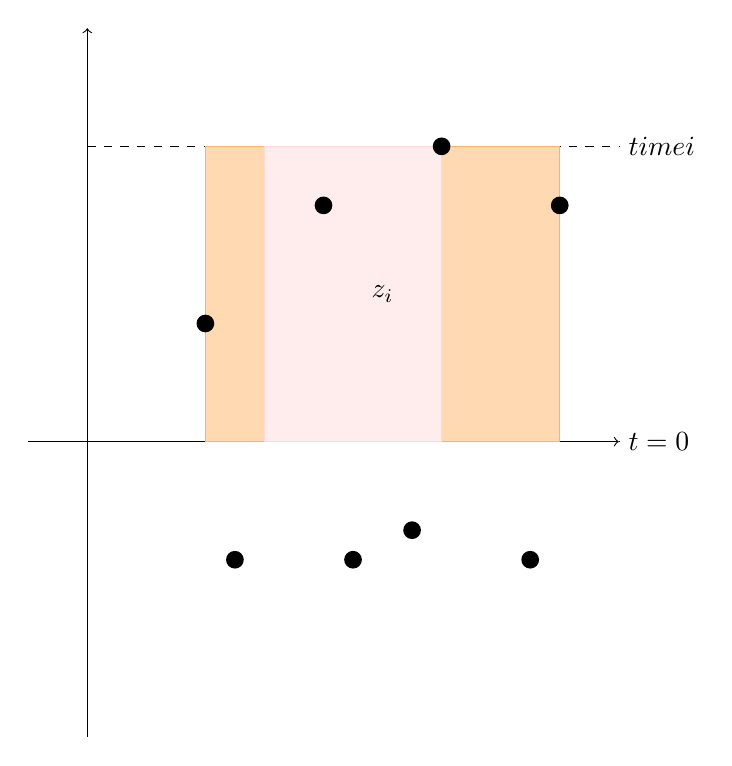
\begin{tikzpicture}[scale=1.5]
    % Draw the axes
    \draw[->] (-0.5,0) -- (4.5,0);
    \draw[->] (0,-2.5) -- (0,3.5);

    % Dashed lines
    \draw[dashed] (0,2.5) -- (4.5,2.5) node[right] {$\text{time } i$};
    \draw[dashed] (0,0) -- (4.5,0) node[right] {$t=0$};

    % Arrows
    \fill[orange!30, draw=orange!60] (1,0) rectangle (2.5,2.5) (2.5,0) rectangle (4,2.5);
    \fill[pink!30, draw=pink!60] (1.5,0) rectangle (3,2.5);

    % Points at time i
    \foreach \x/\y/\color in {1/1/red, 2/2/blue, 3/2.5/blue, 4/2/red} {
        \fill[\color] (\x,\y) circle (0.075);
    }

    % Points from the initial tree
    \foreach \x/\y/\color in {1.25/-1/blue!50, 2.75/-0.75/blue!50, 2.25/-1/white, 3.75/-1/white} {
        \fill[\color] (\x,\y) circle (0.075);
    }

    % Label z_i
    \node at (2.5, 1.25) {$z_i$};
\end{tikzpicture}
\end{document}